\chapter{Das Lebesgue-Maß}
  \begin{lemma}
    Der elementargeometrische Inhalt $vol^n: \script{Q}^n \to [0, \infty]$ ist ein Prämaß auf dem Halbring $\script{Q}^n$ im $\mathbb{R}^n$
  \end{lemma}

  \begin{proof}
    Sei $P = \bigcup\limits_{i=1}^{\infty}P_i$ mit $P_i \cap P_j = \varnothing$ für $i\neq j$, $P$,$P_i \in \script{Q}^n$ $\forall i\in \mathbb{N}$. \newline
    Satz II.27 (i.A. Satz II.26) $\implies vol^n$ ist Inhalt auf Ring $\script{F}^n  \implies \sum\limits_{i=1}^{\infty}vol^n(P_i)$ \newline $= \lim\limits_{k\to\infty}\sum\limits_{i=1}^{k}vol^n(P_i) = \lim\limits_{k\to\infty}vol^n(\bigcup\limits_{i=1}^{k}P_i) \leq vol^n(P)$. \newline
    Wähle zu $\epsilon > 0$ offene Quader $Q_i \supset P_i$ und einen kompakten Quader $Q \subset P$ mit $\sum\limits_{i=1}^{\infty}vol^n(Q_i) < \sum\limits_{i=1}^{\infty} vol^n(P_i) + \frac{\epsilon}{2}$, $vol^n(P)<vol^n(Q)+\frac{\epsilon}{2}$. \newline
    Satz von Heine-Borel (Satz (XIV).22 Ana1): $Q$ wird von endlich vielen Quadern \newline $Q_i\times ... \times Q_k$ überdeckt ($Q\subset P = \bigcup\limits_{i=1}^{\infty}P_i \subset  \bigcup\limits_{i=1}^{\infty}Q_i$) \newline $\implies vol^n(P) < vol^n(Q) +\frac{\epsilon}{2} \leq \sum\limits_{i=1}^{k}vol^n(Q_i) + \frac{\epsilon}{2} < \sum\limits_{i=1}^{\infty}vol^n(P_i)+\epsilon$. \newline
    Lasse $\epsilon > 0$ $\implies vol^n(P) \leq \sum\limits_{i=1}^{\infty}vol^n(P_i)$. 
  \end{proof}

  \begin{definition}
    Das \textbf{n-dimensionale äußere Lebesgue-Maß} einer Menge $E \subseteq \mathbb{R}^n$ ist definiert durch
    \begin{align*}
      \lambda^n(E) := inf\{\sum\limits_{k \in \mathbb{N}} vol^n(Q_k) \ | \ Q_k \in \script{Q}^n, E \subseteq \bigcup\limits_{k \in \mathbb{N}} Q_k\}
    \end{align*}
    $\lambda^n|_{\script{M}(\lambda^n)}$ ist das \textbf{n-dimensionale Lebesguemaß}.
  \end{definition}

  \begin{remark}
    Bem nach Satz II.31 (i.A. II.30) $\implies$ $\lambda^n$ regulär und vollständig auf $\script{M}(\lambda^n)$
  \end{remark}

  \begin{lemma}
    Betrachte für $k \in \mathbb{N}_0$ die Würfelfamilie $\script{W}_k = \{Q_{k,m} := 2^{-k}(m + [0,1]^n) \ | \ m \in \mathbb{R}^n\}$ und definiere für $E \subseteq \mathbb{R}^n$ die Mengen
    \begin{align*}
    F_k(E) := \bigcup \{Q \in \script{W}_k \ | \ Q \subseteq E\} \ \
    F^k(E) := \bigcup \{Q \in \script{W}_k \ | \ Q \cap E \neq \emptyset\}
    \end{align*}
    Dann gilt:
    \begin{enumerate}[label=\roman*)]
      \item $F_k(E)$ und $F^k(E)$ sind abgeschlossene Vereinigungen von abzählbar vielen kompakten Quadern mit paarweise disjunktem Inneren.
      \item $F_1(E) \subseteq F_2(E) \subseteq ... \subseteq E \subseteq ... \subseteq F^2(E) \subseteq F^1(E)$ 
      \item $F_k(E) \supseteq \{x \in \mathbb{R}^n \ | \ dist(x, \mathbb{R}^n \setminus E) > s^{-k} \sqrt{n}\}$\\
      $F^k(E) \subseteq \{x \in \mathbb{R}^n \ | \ dist(x, \mathbb{R}^n \setminus E) \leq s^{-k} \sqrt{n}\}$
      \item $\mathring{E} \subseteq \bigcup\limits_{k \in \mathbb{N}} F_k(E) \subseteq E \ \ \ , \ \ \ \bar{E} \supseteq \bigcap\limits_{k \in \mathbb{N}} F^k(E) \supseteq E$
    \end{enumerate}
  \end{lemma}

  \begin{proof}
    $\bigcup\{Q:Q\in W_k\} = \mathbb{R}^n$ $\forall k\in\mathbb{N}$. \newline
    $W_k$ hat abzählbar viele Elemente, die Würfel aus $W_k$ sind kompakt mit paarweise disjunktem Inneren und jede beschränkte Menge wird nur von endlich vielen Würfeln aus $W_k$ getroffen. $\implies F_k(E)$, $F^k(E)$ sind abgeschlossen $\implies$ i) \newline
    $Q_{k,m}$ ist Vereinigung der $2^n$ Teilwürfel $Q_{k+1, 2m+l}$ mit $l\in \{0,1\}^n$ und es gilt \newline $Q_{k,m} \subset E \implies Q_{k+1, 2m+l} \subset E$ $\forall l\in\{0,1\}^n$ \newline
    $Q_{k+1,2m+l} \cap E \neq \varnothing \implies Q_{k,m} \cap E \neq \varnothing$ wobei $l\in\{0,1\}^n$ \newline
    $\implies F_k(E) \subset F_{k+1}(E)$, $F^k(E) \supset F^{k+1}(E)$ $\implies$ ii) \newline
    Denn für $x \in E$ bel. existiert ein $Q\in W_k$ mit $x\in Q$. \newline
    Sei nun $x\in\mathbb{R}^n$ mit $dist(x,\mathbb{R}^n\setminus E) > 2^{-k}\sqrt{n} \implies \exists Q\in W_k$ mit $x\in Q$ und aus $dist(Q) = 2^{-k}\sqrt{n}$ folgt $Q\subset E \implies x\in F_k(E)\implies \{x\in\mathbb{R}^n: dist(x,\mathbb{R}^n\setminus E) > 2^{-k}\sqrt{n}\} \subset F_k(E)$. \newline
    Ist $x\in F^k(E) \implies \exists Q\in W_k$ mit $x\in Q$ und $Q \cap E \neq \varnothing \implies x\in F^k(E) \implies dist(x,E) \leq dist(Q) \leq 2^{-k}\sqrt{n} \implies$ iii) \newline
    iv) folgt sofort aus iii) und Def. von $\mathring{E}$ bzw. $\bar{E}$. 
    
  \end{proof}

  \sidenote{Vorlesung 9}{30.11.20}
<<<<<<< HEAD
\begin{lemma}
	Die Borelmengen $\script{B}^n$ sind die vom Halbring $\script{Q}^n$ der Quader, dem Ring $\script{F}^n$ der Figuren, und dem System $\script{C}^n$ der abgeschlossenen Mengen des $\mathbb{R}^n$ erzeugten $\sigma$-Algebra, d.h. $\sigma(\script{Q}^n) = \script{B}^n = \sigma(\script{Q}^n) = \sigma(\script{F}^n) = \sigma(\script{C}^n)$
\end{lemma}

\begin{proof}
	Jeder Quader ist Borelmenge: \newline
	Ein Intervall $I\subset \mathbb{R}$ ist entweder offen oder abzählbarer Schnitt von offenen Intervallen und liegt damit in $\script{B}^1$, z.B. $[a,b) = \bigcap\limits_{k=1}^{\infty}(a-\frac{1}{k},b)$. \newline
	Für einen Quader $Q = I_1 \times ... \times I_n \subset \mathbb{R}^n$ schreibe $I_j = \bigcap\limits_{k=1}^{\infty}U_{j,k}$ und damit \newline
	$Q = \bigcap\limits_{k=1}^{\infty}(U_{1,k}\times ... \times U_{n,k}) \in \script{B}^n \implies \script{Q}^n \subset \script{F}^n \subset \script{B}^n$. \newline
	Da Figuren endl. Vereinigungen von Quadern sind und $\script{B}^n$ $\cup$-stabil ist $\implies \sigma(\script{Q}^n) \subset \sigma(\script{F}^n) \subset \script{B}^n$. \newline
	Andererseits folgt aus Lemma III.3, dass $U \subset \mathbb{R}^n$ offen als abzählbare Vereinigung von kompakten Würfeln geschrieben werden kann. \newline
	$\implies \script{O}^n \subset \sigma(\script{Q}^n) \implies \script{B}^n \subset \sigma(\script{Q}^n) \subset \sigma(\script{F}^n)$ \newline 
	$\implies \script{B}^n = \sigma(\script{Q}^n) = \sigma(\script{F}^n)$ \newline
	Abgeschlossene mengen sind Komplemente von offenen Mengen \newline 
	$\implies \sigma(\script{C}^n) = \sigma(\script{O}^n) = \script{B}^n$
\end{proof}

\begin{theorem}
	Für $\lambda^n$ gilt:
	\begin{enumerate}
		\item Alle Borelmengen sind Lebesgue-messbar 
		\item Zu $E \subseteq \mathbb{R}^n \ \exists$ Borelmenge $B \supseteq E$ mit $\lambda^n(B) = \lambda^n(E)$
		\item $\lambda^n(K) < \infty \ \forall K \subseteq \mathbb{R}^n$ kompakt
	\end{enumerate}
\end{theorem}

\begin{proof}
	\item[1] Satz II.31 (i.A. Satz II.30) $\implies \script{Q}^n \subset \script{M}(\lambda^n) \implies \sigma(\script{Q}^n) = \script{B}^n \subset \script{M}(\lambda^n)$ nach Lemma III.4 
	\item[2] Folgt aus Bem. nach Satz II.31 (i.A. Satz II.30)
	\item[3] Es gilt $\lambda^n = vol^n$ auf $\script{Q}^n$ \newline $\implies$ Für $a>0$ bel. ist $\lambda^n([-a,a]^n) = vol^n([-a,a]^n) = (2a)^n < \infty$ $\forall K\subset \mathbb{R}^n$ kompakt $\exists a<\infty: K\subset [-a,a]^n \implies$ Beh.
\end{proof}

\begin{lemma}
	Für $E \subseteq \mathbb{R}^n$ beliebig gilt:
	\begin{enumerate}[label=\roman*)]
		\item $\lambda^n(E) = inf\{\lambda^n(U) \ | \ U \text{ offen }, U \supset E\}$
		\item $\lambda^n(E) = inf\{\lambda^n(K) \ | \ K \text{ kompakt }, K \subset E\}$, falls $E \ \lambda^n$-messbar
	\end{enumerate}
\end{lemma}

\begin{proof}
	\item[i)]Trivial: $\lambda^n(E) \leq inf\{\lambda^n(U): U \text{ offen, } U \supset E\}$\newline
	"$\geq$": O.B. $\lambda^n(E) < \infty$. Def. von $\lambda^n \implies$ Zu $\epsilon > 0$ $\exists$ Überdeckung $E\subset \bigcup\limits_{i=1}^{\infty}P_i$ mit $P_i \in \script{Q}^n$, sodass gilt: $\sum\limits_{i=1}^{\infty}vol^n(P_i) < \lambda^n(E) + \epsilon$. \newline
	O.B. $\forall P_i$ sind offen \newline $\implies U = \bigcup\limits_{i=1}^{\infty}P_i$ offen \newline $\implies E\subset U$ und $\lambda^n(U) \leq \sum\limits_{i=1}^{\infty}vol^n(P_i) < \lambda^n(E) + \epsilon$. 
	\item[ii)] Klar: $\lambda^n(E) \geq sup\{\lambda^n(K): K \text{ kompakt, } K\subset E\}$ \newline "$\leq$": \subitem{a)} B beschränkt \newline Wähle $K_0 \subset \mathbb{R}^n$ kompakt mit $E\subset K_0$ $\implies$ Zu $\epsilon > 0$ $\exists U\subset\mathbb{R}^n$ offen mit $U \supset K_0\setminus E$ und $\lambda^n(U) < \lambda^n(K_0\setminus E) + \epsilon = \lambda^n(K_0) - \lambda^n(E) + \epsilon$ \newline Nun ist $K:=K_0\setminus U \subset K_0\setminus (K_0\setminus E) = E$ kompakt \newline $\implies \lambda^n(K) = \lambda^n(K_0) - \lambda^n(K_0\cap U) \geq \lambda^n(K_0) - \lambda^n(U) >  \lambda^n(E) - \epsilon$ \newline
	$\epsilon \to 0 \implies$ Beh.
	\subitem{b)} $E$ $\lambda^n$-messbar beliebig \newline
	Betrachte $E_j := E\cap \{x\in \mathbb{R}^n: ||x||\leq j\}$ $E_j$ beschränkt und $\lambda^n$-messbar \newline
	$\implies \lambda^n(E_j) = sup\{\lambda^n(K): K \text{ kompakt, }K\subset E_j\} \leq sup\{\lambda^n(K): K \text{ kompakt, }K\subset E\}$ \newline
	Aber $\lambda^n(E_j) \to \lambda^n(E)$ mit $j\to\infty$ nach Satz I.7 $\implies$ Beh.
	
	
\end{proof}
\begin{theorem}
	$D \subseteq \mathbb{R}^n$ ist genau dann $\lambda^n$-messbar, wenn eine der beiden Bedingungen gilt:
	\begin{enumerate}[label=\roman*)]
		\item $\exists$ Borlemenge $E \supset D$ mit $\lambda^n(E \setminus D) = 0$
		\item $\exists$ Borlemenge $C \subset D$ mit $\lambda^n(D \setminus C) = 0$
	\end{enumerate}
	Es kann $E = \bigcap\limits_{i \in \mathbb{N}} U_i$ mit $U_i$ offen und $C = \bigcup\limits_{j \in \mathbb{N}} A_j$ mit $A_j$ abgeschlossen gewählt werden.
\end{theorem}

\begin{proof}
	Äquivalenz von i) bzw. ii) mit $\lambda^n$-Messbarkeit von (?) wurde in Lemma II.18 (i.A. Lemma II.17) gezeigt. \newline
	Sei $D$ $\lambda^n$-messbar. Schreibe $D = \bigcup\limits_{j=1}^{\infty}D_j$ mit $D_j = \{x\in D: j-1 \leq ||x|| < j\}$ \newline
	Lemma III.6 $\implies \exists U_{i,j}$ offen bzw. $K_{i,j}$ kompakt mit $U_{i,j} \supset D_j \supset K_{i,j}$ und \newline $\lambda^n(U_{i,j}) <  \lambda^n(D_j) + \frac{2^{-j}}{i}$, $\lambda^n(K_{i,j}) > \lambda^n(D_j)-\frac{2^{-j}}{i}$ \newline
	$\implies U_i := \bigcup\limits_{j=1}^{\infty}U_{i,j}$ offen und $A_i := \bigcup\limits_{j=1}^{\infty}K_{i,j}$ abgeschlossen ($K_{i,j}\cap K_{i,m} = \varnothing$ for $j\neq m$) \newline
	und es gilt: $U_i \supset D \supset A_i$ \newline
	Mit $E:=\bigcap\limits_{i=1}^{\infty}U_i$, $C:=\bigcup\limits_{i=1}^{\infty}A_i$ gelten für $i\in\mathbb{N}$: \newline
	$\lambda^n(E\setminus D) \leq \lambda^n(U_i\setminus D) \leq \sum\limits_{j=1}^{\infty}\lambda^n(U_{i,j}\setminus D_j) = \sum\limits_{j=1}^{\infty}(\lambda^n(U_{i,j})-\lambda^n(D_j)) \leq \frac{1}{i}$ \newline
	$\lambda^n(D\setminus C) \leq \lambda^n(D\setminus A_i) \leq \sum\limits_{j=1}^{\infty}\lambda^n(D_j\setminus K_{i,j}) = \sum\limits_{j=1}^{\infty}(\lambda^n(D_j) - \lambda^n(K_{i,j})) \leq \frac{1}{i}$ \newline
	Mit $i\to\infty$ folgt Beh. 
\end{proof}
\newpage

\begin{theorem}[Satz von Lusin]
	Sei $A \subseteq \mathbb{R}^n$ offen mit $\lambda^n(A) < \infty$ und sei $f \ \lambda^n$-messbar auf $A$ mit Werten in $\mathbb{R}$. Dann existiert $\forall \epsilon > 0$ ein $K = K_{\epsilon} \subseteq A$ kompakt, mit:
	\begin{enumerate}[label=\roman*)]
		\item $\lambda^n(A \setminus K) < \epsilon$
		\item $f|_k$ ist stetig
	\end{enumerate}
\end{theorem}

\begin{proof}
	Kap II. $\implies$ oBdA ist $f$ auf ganz $A$ definiert, d.h. $f: A\to \mathbb{R}$. Für $i\in\mathbb{N}$ setze \newline
	$B_{i(2k+1)}:=[\frac{k}{i}, \frac{k+1}{i}]$, $k\in\mathbb{N}_0$ \newline
	$B_{i(2k)} := [-\frac{k}{i}, -\frac{k-1}{i}]$, $k\in\mathbb{N}_0$ \newline
	$B_{i(j)}$, $j\in\mathbb{N}_0$, sind paarweise disjunkt mit $\bigcup\limits_{j\in\mathbb{N}_o} B_{i(j)} = \mathbb{R}$ und (?)($B_{i(j)} = \frac{1}{i}$)\newline
	$A_{i,j} := f^{-1}(B_{i(j)})$ sind $\lambda^n$-messbar und $A = \bigcup\limits_{j\in\mathbb{N}_0}A_{ij}$. \newline
	Lemma III.6 ii) $\implies \exists K_{ij} \subset A_{ij}$ kompakt mit $\lambda^n(A_{ij\setminus K_{ij}}) < \frac{\epsilon}{2^{i+j}}$ \newline
	$\implies \lambda^n(A\setminus \bigcup\limits_{l=1}^{\infty}K_{il}) = \lambda^n(\bigcup\limits_{j=1}^{\infty} A_{ij} \setminus \bigcup\limits_{l=1}^{\infty}K_{il}) \leq \lambda^n(\bigcup\limits_{j=1}^{\infty}(A_{ij}\setminus K_{ik})) < \frac{\epsilon}{2^i}$ \newline
	Satz I.7 ii) $\implies \lim\limits_{N\to\infty} \lambda^n(A\setminus \bigcup\limits_{l=1}^{N}K_{il}) = \lambda^n(A\setminus \bigcup\limits_{l=1}^{\infty}K_{il}) < \frac{\epsilon}{2^i}$ \newline
	$\implies \exists N(i)$ mit $\lambda^n(A\setminus \bigcup\limits_{j=1}^{N(i)}K_{ij}) < \frac{\epsilon}{2^i}$ \newline
	$\implies D_i := \bigcup\limits_{j=1}^{N(i)}K_{ik}$ ist kompakt. \newline
	$\forall i,j$ wählen wir $b_{ij}\in B_{i(j)}$ und definiere $g_i: D_i \to \mathbb{R}$ durch $g_i(x) := b_{ij}$ $\forall x\in K_{ij}$ ($j \leq N(i)$) \newline 
	$K_{i1}, ...,K_{iN(i)}$ sind kompakt, paarweise disjunkt \newline 
	$\implies$ Sie haben positiven Abstand voneinander \newline
	$\implies g_i$ ist stetig \newline
	Aus Konstruktion folgt \begin{equation}
	|f(x) - g_i(x)| \leq \frac{1}{i} \text{ } \forall x\in D_i
	\label{eq1}
	\end{equation}
	Setze $K:= \bigcap\limits_{i=1}^{\infty} D_i \implies K$ ist kompakt und $\lambda^n(A\setminus K) \leq \sum\limits_{i=1}^{\infty}\lambda^n(A\setminus D_i) < \epsilon$ \newline
	Aus \ref{eq1} und Def von $K$ folgt: $g_i$ konvergiert gleichmäßig gegen $f$ auf $K$ $\implies f$ ist stetig auf $K$. 
	\end{proof}
=======

  \begin{lemma}
    Die Borelmengen $\script{B}^n$ sind die vom Halbring $\script{Q}^n$ der Quader, dem Ring $\script{F}^n$ der Figuren, und dem System $\script{C}^n$ der abgeschlossenen Mengen des $\mathbb{R}^n$ erzeugten $\sigma$-Algebra, d.h. $\sigma(\script{Q}^n) = \script{B}^n = \sigma(\script{Q}^n) = \sigma(\script{F}^n) = \sigma(\script{C}^n)$
  \end{lemma}

  \begin{proof}
    siehe Aufschrieb
  \end{proof}

  \newpage
  \begin{theorem}
    Für $\lambda^n$ gilt:
    \begin{enumerate}
      \item Alle Borelmengen sind Lebesgue-messbar 
      \item Zu $E \subseteq \mathbb{R}^n \ \exists$ Borelmenge $B \supseteq E$ mit $\lambda^n(B) = \lambda^n(E)$
      \item $\lambda^n(K) < \infty \ \forall K \subseteq \mathbb{R}^n$ kompakt
    \end{enumerate}
  \end{theorem}

  \begin{proof}
    siehe Aufschrieb
  \end{proof}

  \begin{lemma}
    Für $E \subseteq \mathbb{R}^n$ beliebig gilt:
    \begin{enumerate}[label=\roman*)]
      \item $\lambda^n(E) = inf\{\lambda^n(U) \ | \ U \text{ offen }, U \supset E\}$
      \item $\lambda^n(E) = inf\{\lambda^n(K) \ | \ K \text{ kompakt }, K \subset E\}$, falls $E \ \lambda^n$-messbar
    \end{enumerate}
  \end{lemma}

  \begin{theorem}
    $D \subseteq \mathbb{R}^n$ ist genau dann $\lambda^n$-messbar, wenn eine der beiden Bedingungen gilt:
    \begin{enumerate}[label=\roman*)]
      \item $\exists$ Borlemenge $E \supset D$ mit $\lambda^n(E \setminus D) = 0$
      \item $\exists$ Borlemenge $C \subset D$ mit $\lambda^n(D \setminus C) = 0$
    \end{enumerate}
    Es kann $E = \bigcap\limits_{i \in \mathbb{N}} U_i$ mit $U_i$ offen und $C = \bigcup\limits_{j \in \mathbb{N}} A_j$ mit $A_j$ abgeschlossen gewählt werden.
  \end{theorem}

  \newpage

  \begin{theorem}[Satz von Lusin]
    Sei $A \subseteq \mathbb{R}^n$ offen mit $\lambda^n(A) < \infty$ und sei $f \ \lambda^n$-messbar auf $A$ mit Werten in $\mathbb{R}$. Dann existiert $\forall \epsilon > 0$ ein $K = K_{\epsilon} \subseteq A$ kompakt, mit:
    \begin{enumerate}[label=\roman*)]
      \item $\lambda^n(A \setminus K) < \epsilon$
      \item $f|_k$ ist stetig
    \end{enumerate}
  \end{theorem}
>>>>>>> 4b16f17268042f1a800025c4c38bcc4482ee1a05

  \sidenote{Vorlesung 10}{4.12.20}

  \begin{definition}
    Ein äußeres Maß $\mu$ auf $\mathbb{R}^n$ heißt \textbf{Borelmaß}, falls gilt:
    \begin{enumerate}
      \item Alle Borelmengen sind $\mu$-messbar
      \item $\mu(K)<\infty \ \forall K \subseteq \mathbb{R}^n$ kompakt
    \end{enumerate}
  \end{definition}

  \begin{remark}
    $\lambda^n$ ist Borelmaß nach Satz III.5.\\
    Ein äußeres Maß $\mu$ auf $\mathbb{R}^n$ heißt \textbf{translationsinvariant}, falls \\
    $\mu(E + a) = \mu(E) \ \forall E \subset \mathbb{R}^n, a \in \mathbb{R}^n$ mit $E + a := \{x + a \ | \ x \in E\}$\\
    Bemerke: $vol^n:\script{Q}^n \to [0, \infty]$ ist translationsinvariant $\implies$ $\lambda^n$ ist translationsinvariant.
  \end{remark}

  \begin{lemma}
    Ist $\mu$ translationsinvariantes Borelmaß auf $\mathbb{R}^n$, so ist jede Koordinaten-Hyperebene $H := \{x \in \mathbb{R}^n \ | \ x_i = c\} (i=1,...,n)$ eine $\mu$-Nullmenge.
  \end{lemma}

  \begin{proof}
      Sei $Q = [0,1]^n$ und $F = \{x\in Q: x_i = 0\}$. Für $a\in\mathbb{R}^n$ ist $F+a$ abgeschlossen $\implies$ $\mu$-messbar. Für $\{s_i, ..., s_k\} \subset [0,1]$ folgt: \newline $k\mu(F) = \sum\limits_{j=1}^{k}\mu(s_j e_i + F) = \mu(\bigcup\limits_{j=1}^{k}(s_j e_i + F)) \leq \mu(Q) < \infty$  \newline
$k$ kann beliebig groß gewählt werden $\implies \mu(F) = 0$. \newline
$H$ ist Vereinigung abzählbar vieler Translationen von $F \implies \mu(H) = 0$
  \end{proof}

  \begin{theorem}
    Sei $\mu$ translationsinvariantes Borelmaß auf $\mathbb{R}^n$. Dann gilt mit $\theta := \mu([0,1]^n)$:
    \begin{align*}
      \mu(E) = \theta \lambda^n(E) \ \ \ \ \forall \ \lambda^n \text{-messbaren } E \subseteq \mathbb{R}^n
    \end{align*}
  \end{theorem}

    \begin{proof}
	Setze $Q_{k,j} = 2^{-k}(j+[0,1]^n)$ für $k\in\mathbb{N}_0$, $j\in\mathbb{R}^n \implies [0,1]^n$ ist Vereinigung der $2^{nk}$ abgeschlossenen Teilwürfel $\{Q_{k,j}: j\in J_k\}$ mit $J_k = \{j = (j_1, ...., j_n) \in \mathbb{R}^n: 0$ $leq j_i \leq 2^k-1\}$ mit paarweise disjunktem Inneren. Lemma III.10 \newline  $\implies \mu([0,1]^n) = \sum\limits_{j\in J_k} \mu(Q_{k,j})$ \newline
	$\lambda^n([0,1]^n) = \sum\limits_{j\in J_k} \lambda^n(Q_{k,j})$ \newline
	Translationsinvarianz $\implies \mu(Q{k,j}) = \mu(Q_{k,0})$ \newline
	$\lambda^n(Q_{k,j}) = \lambda^n(Q_{k,0})$ $\forall  j\in \mathbb{R}^n$ \newline
	$\implies \theta = \frac{\mu([0,1]^n)}{\lambda^n([0,1]^n)} = \frac{\mu(Q_{k,0})}{\lambda^n(Q_{k,0})} = \frac{\mu(Q_{k,j})}{\lambda^n(Q_{k,j})}$ $\forall j\in \mathbb{R}^n$ \newline
	Lemma III.3, Lemma III.10 $\implies \mu(U) = \theta \lambda^n(U)$ $\forall U\supset \mathbb{R}^n$ offen \newline
	$\implies$ Beh. gilt für alle $Q \in \script{Q}^n$ und damit $\forall$ $\lambda^n$-messbaren Teilmengen nach Eindeutigkeit der Massfortsetzung, Satz II.17 (i.A. Satz II.16). 
\end{proof}

  \begin{lemma}
    $U \subseteq \mathbb{R}^n$ offen, $f: U \to \mathbb{R}^n$ lipschitz-stetig mit Konstante $\Lambda$ bzgl. $||.||_{\infty}$. Dann gilt:
    \begin{align*}
      \lambda^n(f(E)) \leq \Lambda^n \lambda^n(E) \ \ \ \ \forall E \subseteq U
    \end{align*}
  \end{lemma}

    \begin{proof}
	O.E. $\lambda^n(E) < \infty$ \newline
	Setze $Q_{\rho}(x_0) = \{x\in\mathbb{R}^n: ||x-x_0||_{\infty} < \rho\}$ $\forall x_0\in\mathbb{R}^n$, $\rho >0$ \newline
	Vor $\implies ||f(x)-f(x_0)||_{\infty} \leq \Lambda ||x-x_0||_{\infty}$ für $x,x_0\in U$ \newline
	Also $Q_{\rho}(x_0) \subset U \implies f(Q_{rho}(x_0)) \subset Q_{\Lambda \rho}(f(x_0))$ \newline
	Lemma III.6 $\implies$ $\exists V$ offen mit $E\subset V$ und $\lambda^n(V) < \lambda^n(E) + \epsilon$ $\forall$ $\epsilon >0$. \newline
	(O.E. $V\subset U$) \newline 
	Weiter existiert $Q_j$ Würfel mit paarweise disjunktem Inneren und $V = \bigcup\limits_{j=1}^{\infty}Q_j$ \newline
	$\implies \lambda^n(f(E)) \leq \lambda^n(f(V)) \leq \sum\limits_{j=1}^{\infty}\lambda^n(f(Q_j)) \leq \Lambda^n \sum\limits_{j=1}^{\infty}\lambda^n(Q_j) \leq \Lambda^n(\lambda(E)+\epsilon)$ \newline
	Lasse $\epsilon\to 0 \implies$ Beh. 
\end{proof}

  \begin{theorem}
    $U \subseteq \mathbb{R}^n$ offen und $f \in C^1(U, \mathbb{R}^n)$. Dann gilt:
    \begin{enumerate}
      \item $N \subseteq U$ $\lambda^n$-Nullmenge $\implies$ $f(N)$ $\lambda^n$-Nulllmenge
      \item $E \subseteq U$ $\lambda^n$-messbar $\implies$ $f(E)$ $\lambda^n$-messbar
    \end{enumerate}
  \end{theorem}

    \begin{proof}
	Lemma III.3 $\implies U = \bigcup\limits_{i=1}^{\infty}K_i$, $K_i$ kompakte Würfel \newline
	$\implies N = \bigcup\limits_{i=1}^{\infty}K_i\cap N$ \newline
	$f|_K$ ist Lipschitz $\forall$ $K\subset U$ Kpt \newline
	$\implies$ 1) folgt aus Lemma III.12 \newline
	zu 2): O.B. $E$ beschränkt (sonst betrachte $E_m := \{x\in E: ||x||\leq m \}$ $E = \bigcup\limits_{i=1}^{\infty}E_i$)  \newline
	Satz III.7 $\implies \exists$ $A_j$ kompakt und $\lambda^n$-Nullmenge $N$ mit $E=(\bigcup\limits_{j=1}^{\infty}A_j)$ und $f(A_j)$ ist kompakt und $\lambda^n(f(N)) = 0$ nach 1) \newline
	$\implies f(E) = \bigcup\limits_{j=1}^{\infty}f(A_j) \cup f(N)$ $\implies \lambda^n$-messbar
\end{proof}

  \begin{theorem}
    Sei $S \in O(\mathbb{R}^n)$ und $a \in \mathbb{R}^n$, dann gilt:
    \begin{align*}
      \lambda^n(S(E) + a) = \lambda^n(E) \ \ \ \ \forall E \subseteq \mathbb{R}^n
    \end{align*}
  \end{theorem}

    \begin{proof}
	$\lambda^n$ translationsinvariant $\implies$ O.E. $a=0$. \newline
	Sei jetzt $S\in GL(\mathbb{R}^n)$ und $T:=S^{-1}$. \newline
	Definiere $\mu := T(\lambda^n): \script{P}(\mathbb{R}^n) \rightarrow [0,\infty]$, $E \to \mu(E) := \lambda^n(T^{-1}(E))$, d.h.\newline
	$\lambda^n(S(E)) = \mu(E)$. \newline
	Beh.: $\mu$ ist translationsinvariantes Borelmaß. \newline
	Ist $B\subset\mathbb{R}^n$ Borelmenge $\rightarrow B$ $\lambda^n$-messbar (Satz III.5) $\implies T^{-1}(B) = S(B)$ $\lambda^n$-messbar (Satz III.13) $\implies B$ ist $\mu$-messbar (s. Blatt 2) \newline
	Für $K\subset\mathbb{R}^n$ kompakt ist $T^{-1}(K) = S(K)$ kompakt $\implies \mu(K) < \infty \implies \mu$ Borelmaß. \newline
	Sei $b\in\mathbb{R}^n$, $E\subset\mathbb{R}^n$ beliebig \newline 
	$\implies \mu(E+b) = \lambda^n(S(E+b)) = \lambda^n(S(E) + S(b)) = \lambda^n(S(E)) = \mu(E) \implies$ Beh. \newline
	Satz III.11 $\implies \mu(E) = \theta(S) \lambda^n(E)$ $\forall E\subset\mathbb{R}^n$ $\lambda^n$-messbar, wobei $\theta(S) = \mu([0,1]^n) = \lambda^n(S([0,1]^n)) \in [0,\infty]$. \newline
	Für $E\subset\mathbb{R}^n$ bel. gilt mit Lemma III.6 \newline
	$\mu(E) = \lambda^n(S(E)) = inf\{\lambda^n(V): S(E)\subset V \text{ offen}\} = inf\{\lambda^n(S(U)): E\subset U \text{ offen}\}$ \newline $= \theta(S) inf\{\lambda^n(U): E\subset U \text{ offen}\}$ \newline
	$\implies \mu(E) = \lambda^n(S(E)) = \theta(S) \lambda^n(E)$ $\forall E\subset\mathbb{R}^n$ \newline
	Ist $S\in O(\mathbb{R}^n)$, so wähle $E = B_1(O) \implies S(B_1(O) = B_1(O))$ \newline
	$\implies \mu(B_1(O)) = \lambda^n(B_1(O)) \implies \theta(S) = 1$ $\forall S\in O(\mathbb{R}^n)$ \newline
	$\implies \lambda^n(S(E)) = \lambda^n(E)$ $\forall S \in O(\mathbb{R}^n)$
\end{proof}

  \begin{lemma}[Polarzerlegung]
    $\forall S \in GL(\mathbb{R}^n) \ \exists$ Diagonalmatrix $\Lambda$ mit Einträgen $\lambda_i > 0, i=1,...,n$ und \\
    $T_1, T_2 \in O(\mathbb{R}^n)$, sodass $S = T_1 \Lambda T_2$ 
  \end{lemma}

    \begin{proof}
	$S^T S$ ist symmetrisch und hat positive EW, denn für \newline $v\in\mathbb{R}^n\setminus\{0\}:$ $<S^T Sv,v > = ||Sv||^2 > 0$ \newline
	$\implies \exists T\in O(\mathbb{R}^n)$ und $\Lambda$ Diagonalmatrix mit Einträgen $\lambda_i > 0$ $i=1,...,n$, sodass $S^T S = T \Lambda^2 T^{-1}$. \newline
	$R := T \Lambda T^{-1}$ ist symmetrisch mit $R^2 = S^T S$ $\implies$ mit $Q := S R^{-1}$ gilt \newline
	$Q^T Q = (R^{-1})^T S^T S R^{-1} = R^{-1} R^2 R^{-1} = \mathbb{I}_n \implies Q \in O(\mathbb{R}^n)$ \newline
	$\implies S = Q R = Q T \Lambda T^{-1} = T_1 \Lambda T_2$ mit $T_1 := Q T \in O(\mathbb{R}^n)$, $T_2 := T^{-1} \in O(\mathbb{R}^n)$
	\end{proof}

  \begin{theorem}[Lineare Transformationsformel]
    Für eine lineare Abbildung $S: \mathbb{R}^n \to \mathbb{R}^n$ gilt:
    \begin{align*}
      \lambda^n(S(E)) = |det(S)| \ \lambda^n(E) \ \ \ \ \forall E \subseteq \mathbb{R}^n
    \end{align*}
  \end{theorem}

    \begin{proof}
	Ist $det(S) = 0 \implies S(E)$ liegt in Hyperebene $\implies$ Beh. folgt aus Lemma III.10. \newline
	Ist $det(S) \neq 0 \implies$ (*) aus Beweis von Satz III.14, d.h. $\lambda^n(S(E)) = \theta(S) \lambda^n(E)$ \newline
	z.z. $\theta(S) = |det(S)|$ \newline
	i) S diagonal mit Einträgen $\lambda_i > 0 \implies \theta(S) = \lambda^n(S([0,1]^n)) = \lambda^n([0,\lambda_1]\times ... \times [0,\lambda_n])= \Pi_{i=1}^{n} \lambda_i = |det(S)|$ \newline 
	ii) $S\in GL(\mathbb{R}^n)$ bel. $\implies S = T_1 \Lambda T_2$ s.Lemma III.15, $T_1$, $T_2 \in O(\mathbb{R}^n)$ \newline
	$\implies \theta(S) = \lambda^n(T_1\Lambda T_2([0,1]^n)) = \lambda^n(\Lambda T_2([0,1]^n)) = |det(\Lambda)| \lambda^n(T_2([0,1]^n))$ \newline $= |det(\Lambda)| \lambda^n([0,1]^n) = |det(S)|$
	\end{proof}

  \begin{example}
  \begin{minipage}{0.7\textwidth}
    $\lambda_1, ...,  \lambda_n > 0, \ E=\{x \in \mathbb{R}^n \ | \ (\dfrac{x_1}{\lambda_1})^2 + ... + (\dfrac{x_n}{\lambda_n})^2 < 1\}$\\
    mit $\Lambda = \begin{pmatrix}
      \lambda_1 & &\\
      & \ddots &\\
      & & \lambda_n
    \end{pmatrix}
    \in GL(\mathbb{R}^n)$ gilt $E = \Lambda(B_1(0))$\\
    Satz III.16 $\implies \lambda^n(E) = \lambda^n(\Lambda(B_1(0))) = \lambda_1 \cdot ... \cdot \lambda_n \cdot \lambda^n(B_1(0))$
  \end{minipage}\hfill
  \begin{minipage}{0.3\textwidth}
    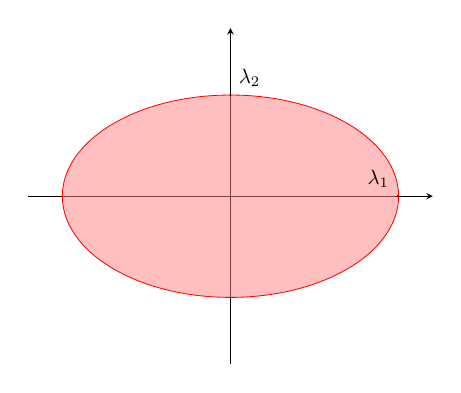
\begin{tikzpicture}[scale=.75]
      \begin{axis}[
        xmin=-2, xmax=2,
        ymin=-2, ymax=2,
        xtick=\empty,
        ytick=\empty,
        axis lines=middle,
        ]
        \draw[red, fill=red!50, fill opacity=0.5] (axis cs:0,0) ellipse [rotate=90, x radius=1, y radius=2];
        \node[label={45:{$\lambda_2$}},circle,fill,inner sep=0pt] at (axis cs:0,1.2) {};
        \node[label={135:{$\lambda_1$}},circle,fill,inner sep=0pt] at (axis cs:1.65,0) {};
      \end{axis}
    \end{tikzpicture}
  \end{minipage}
  \end{example}

\sidenote{Vorlesung 11}{04.12.2020}
  \begin{example}[Vitali 1905]
    $\script{P}(\mathbb{R}^n) \neq \script{M}(\lambda^n)$\\
    Beweis siehe Aufschrieb.
  \end{example}

  